\chapter{Desenvolvimento}
\label{chap:desenvolvimento}

Nesta seção serão demonstrados os trabalhos realizados durante o período do curso de formação em Robótica e Sistemas Autônomos, identificando nos Apêndices os relatórios e estudos gerados. 


\section{\textit{Husky} com missão de busca da bola amarela- Desafio 1.0 }
\label{sec:desafio_1}
Este desafio foi feito individualmente, e ele foi realizado com o objetivo de programar o robô da \textit{Clearpath Robotics- Husky}, no ambiente de simulação do \textit{Gazebo}. A área de operação desse robô foi a área externa entre os prédios do CIMATEC 3 e 4. O \textit{Husky} tinha como missão explorar esse ambiente externo a procura de uma bola amarela, e ao identificar esta ele deveria ir até ela e parar de frente para mesma informando que a missão foi completada. Como nesse desafio foi realizada apenas a simulação, apenas o computador foi utilizado.  


% \begin{figure}[H]
%     \caption{Área externa do CIMATEC 3 e 4, ambiente de simulação do \textit{Gazebo}}
%     \centering
%     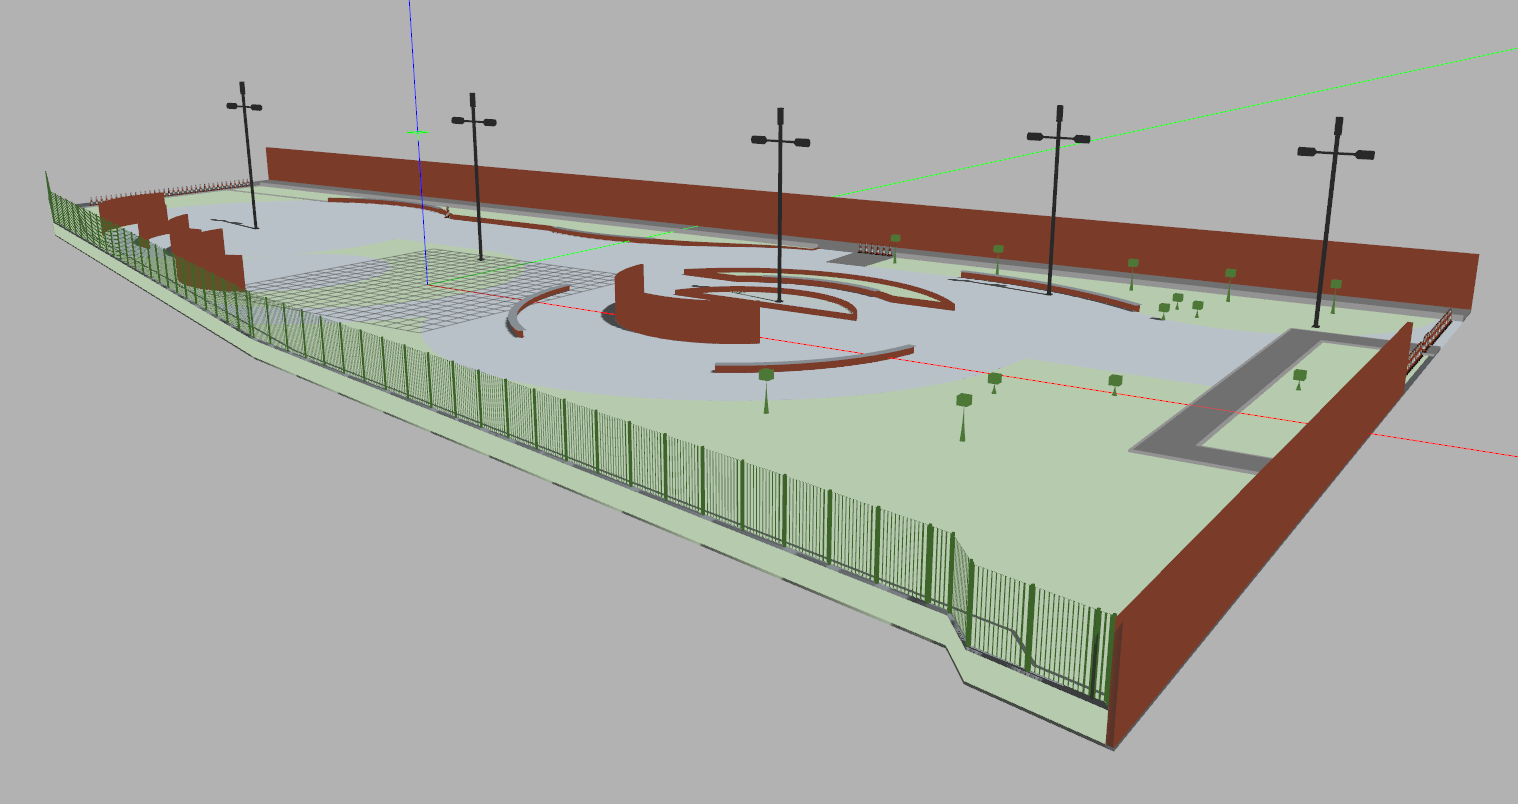
\includegraphics[width= \textwidth]{Figures/cimatec4.png}
%     \caption*{Fonte: Grupo de Formação em Robótica e Sistemas Autônomos}
%     \label{fig:cimatec3_4}
% \end{figure}


\section{Relatório Parcial do Manipulador TIMON-HM- Desafio 2.0 }
%\section{Desafio 2.0 }
\label{sec:desafio_2}
O segundo desafio foi realizado em grupo, onde um manipulador, TIMON-HM, deveria ser concebido desde sua fase inicial modelando toda sua estrutura e posteriormente realizada a simulação deste no \textit{Gazebo}, com a missão da câmera integrada ao manipulador identificar o \textit{tag ArUco} na caixa e pressionar o botão. Este desafio também foi realizada apenas a simulação. No Apêndice \ref{append:timon} encontra-se o relatório elaborado para esse desafio, com todas as especificações do mesmo, o estado da arte, metodologia e materiais utilizados.

% \begin{figure}[H]
%     \caption{Realização do desafio no ambiente de simulação do \textit{Gazebo}}
%     \centering
%     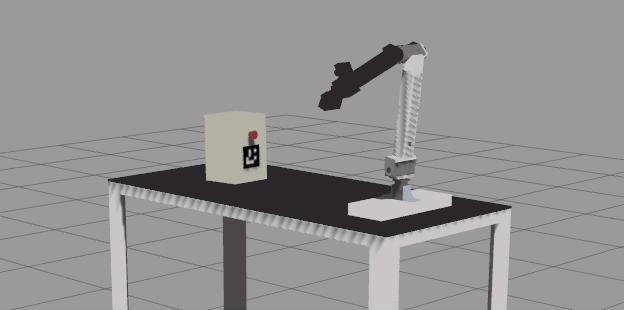
\includegraphics[width= \textwidth]{Figures/manipulador_simulacao.png}
%     \caption*{Fonte: Grupo de Formação em Robótica e Sistemas Autônomos}
%     \label{fig:manipulador_simulacao}
% \end{figure}


\section{Resultado do Manipulador Robótico JeRoTIMON- Desafio 2.2 }
%\section{Desafio 2.2 }
\label{sec:desafio_2_2}
Este desafio foi para construir o modelo real do manipulador JeRoTIMON modelado e simulado no desafio \ref{sec:desafio_2}, realizado em grupo, onde o objetivo era o mesmo, reconhecer a \textit{tag ArUco} na caixa e pressionar o botão, só que dessa vez no ambiente real. Os materiais utilizados nesse desafio foram perfis de alumínio, motores \textit{Dynamixel}, câmera RGB modelo \textit{Teledyne Genie Nano C2590},  peças modeladas no \textit{OnShape} e impressas em \textit{ABS} por uma impressora 3D, conexões para alimentação e para comunicação.
No Apêndice \ref{append:jerotimon} está disponível o relatório gerado para esse projeto, para maiores detalhes.



% \begin{figure}[H]
%     \caption{Realização do desafio no ambiente real}
%     \centering
%     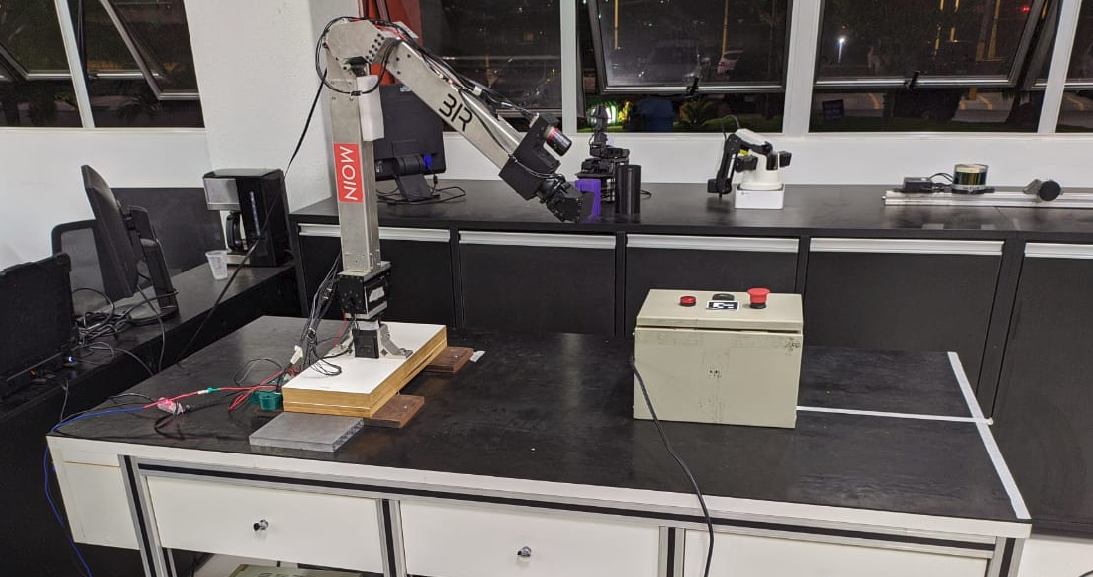
\includegraphics[width= \textwidth]{Figures/manipulador_real.png}
%     \caption*{Fonte: Grupo de Formação em Robótica e Sistemas Autônomos}
%     \label{fig:manipulador_real}
% \end{figure}


\section{Analíse estatística R\&R da simulação do robô Darwin OP- Desafio 2.5}
%\section{Desafio 2.5}
\label{sec:desafio_2_5}
O desafio 2.5 foi realizado em equipe, a mesma do desafio \ref{sec:desafio_2}, onde o robô programado foi o \textit{Darwin-OP} e este deveria realizar duas missões, a primeira, é a marcha, onde quatro robôs \textit{Darwin-OP} deveriam andar de forma sincronizada de um ponto a outro da pista de corrida. E a segunda missão foi realizada a programação para que os quatro robôs realizassem a corrida com revezamento, onde cada robô está posicionado numa parte específica da pista de corrida e ao chegar próximo um do outro eles mantém por um período a movimentação sincronizada depois o anterior para e o outro segue, igualmente a uma corrida com revezamento real.

Sobre esse projeto foi realizado um estudo que teve como objetivo analisar o sistema de medição dos dados coletados durante os testes realizados nas etapas: de marcha e de revezamento, utilizando o método de análise de variância (ANOVA). Nessa análise foi possível aplicar os conhecimentos obtidos em estatística, utilizando a ferramenta e linguagem de programação \textit{R} em um projeto realizado durante o curso, a fim de verificar o desempenho desse projeto, exemplo, a análise de precisão produzida através do estudo R\&R (Repetibilidade e Reprodutibilidade). Foram utilizadas apenas as ferramentas de simulação e para realização do estudo estatístico.
O resultado proveniente deste estudo está descrito no documento Avaliação do Sistema de Medição- TIMON 2.5 no Apêndice \ref{append:darwinop}. Onde estão expostos dos dados coletados e a interpretação dos resultados obtidos.
% Na Figura \ref{fig:marcha_darwinop} tem-se os robôs executando a programação da marcha, e na Figura \ref{fig:revezamento_darwinop} tem-se os robôs executando o código do revezamento. No Apêndice \ref{append:readme_darwinop} está o \textit{Read me} do repositório.



% \begin{figure}[H]
%     \caption{Simulação do Desafio 2.5- Marcha}
%     \centering
%     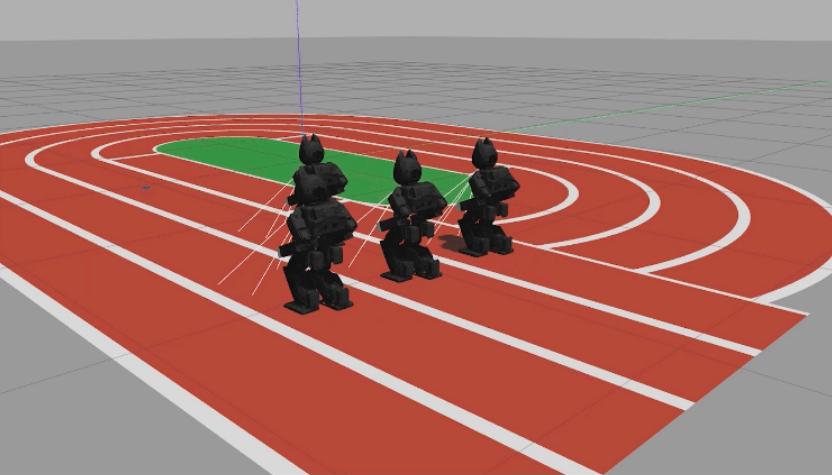
\includegraphics[width= \textwidth]{Figures/marcha.png}
%     \caption*{Fonte: Grupo de Formação em Robótica e Sistemas Autônomos}
%     \label{fig:marcha_darwinop}
% \end{figure}



% \begin{figure}[H]
%     \caption{Simulação do Desafio 2.5- Revezamento}
%     \centering
%     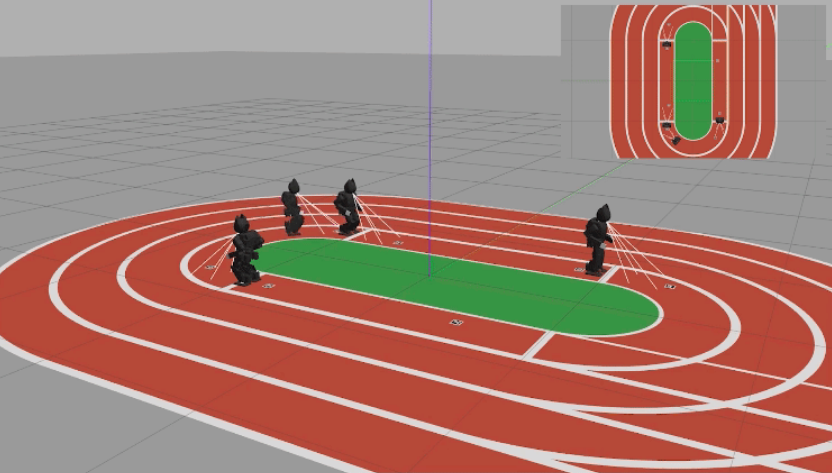
\includegraphics[width= \textwidth]{Figures/revezamento.png}
%     \caption*{Fonte: Grupo de Formação em Robótica e Sistemas Autônomos}
%     \label{fig:revezamento_darwinop}
% \end{figure}

\section{Planejamento de Experimentos (DOE) -Helicóptero de Papel (TIMON-HM)}
%\section{Planejamento de Experimentos (DOE)- Helicóptero de Papel (TIMON-HM)}
\label{sec:analise_doe}
Esse experimento teve como objetivo aplicar os conceitos de Planejamento de Experimento- \textit{DOE}, a um modelo de helicóptero de papel. O propósito principal foi identificar quais são os fatores que mais influenciam seu tempo de voo e como estas variáveis podem melhorar o seu desempenho. Durante o processo, foi utilizado um modelo de helicóptero em papel onde foi medido o seu tempo de voo em duas alturas diferentes, além disto, foram adicionados adesivos e um clipe em sua estrutura a fim de verificar a influência da variação destes parâmetros no resultado final. Esse estudo proporcionou a aplicação do aprendizado adquirido ao uso da ferramenta e linguagem R usada para manipulação, análise e visualização de dados, e dos conhecimentos de Estatística. 
Esse estudo resultou no relatório Planejamento de Experimentos (DOE) -Helicóptero de Papel (TIMON-HM) disponível no Apêndice \ref{append:doe}, onde neste consta informações sobre o que é o \textit{DOE}, como e qual o motivo da escolha dos fatores de influência e os níveis e os resultados obtidos. 



\section{UGV SACI: Integrado com Detecção Visual e Manipulador- Desafio 3.0}
%\section{Desafio 3.0}
\label{sec:desafio_3_0}
Neste desafio foi desenvolvido o Saci, que integra o veículo autônomo da \textit{Clearpath Robotics Warthog} equipado com sensores (câmeras, LiDAR e GPS) e o manipulador robótico JeRoTIMON, com o propósito de transformá-lo em um robô autônomo. Este foi construído com o intuito de que o mesmo tivesse navegação autônoma para realizar investigação em ambiente externo e construir um mapa deste ambiente, detectasse a "bomba" escondida, e realizasse o desarme da bomba através do manipulador. 
Esse projeto foi desenvolvido em duas etapas, a de simulação, onde foram utilizados o software  \textit{Gazebo} e a ferramenta de visualização \textit{Rviz}, e para configuração do pacote de parâmetros do manipulador foi utilizado \textit{MoveIt}. E em paralelo foi desenvolvido este robô em sua versão real, onde foi possível realizar testes e verificar seu desempenho em campo.

Como resultado obtido desse projeto é possível ver no Apêndice \ref{append:saci}, onde está inserido o relatório gerado para esse projeto.


% \begin{figure}[H]
%     \caption{Ambiente entre os prédios do CIMATEC 3 e 4 na simulação do \textit{Gazebo}}
%     \centering
%     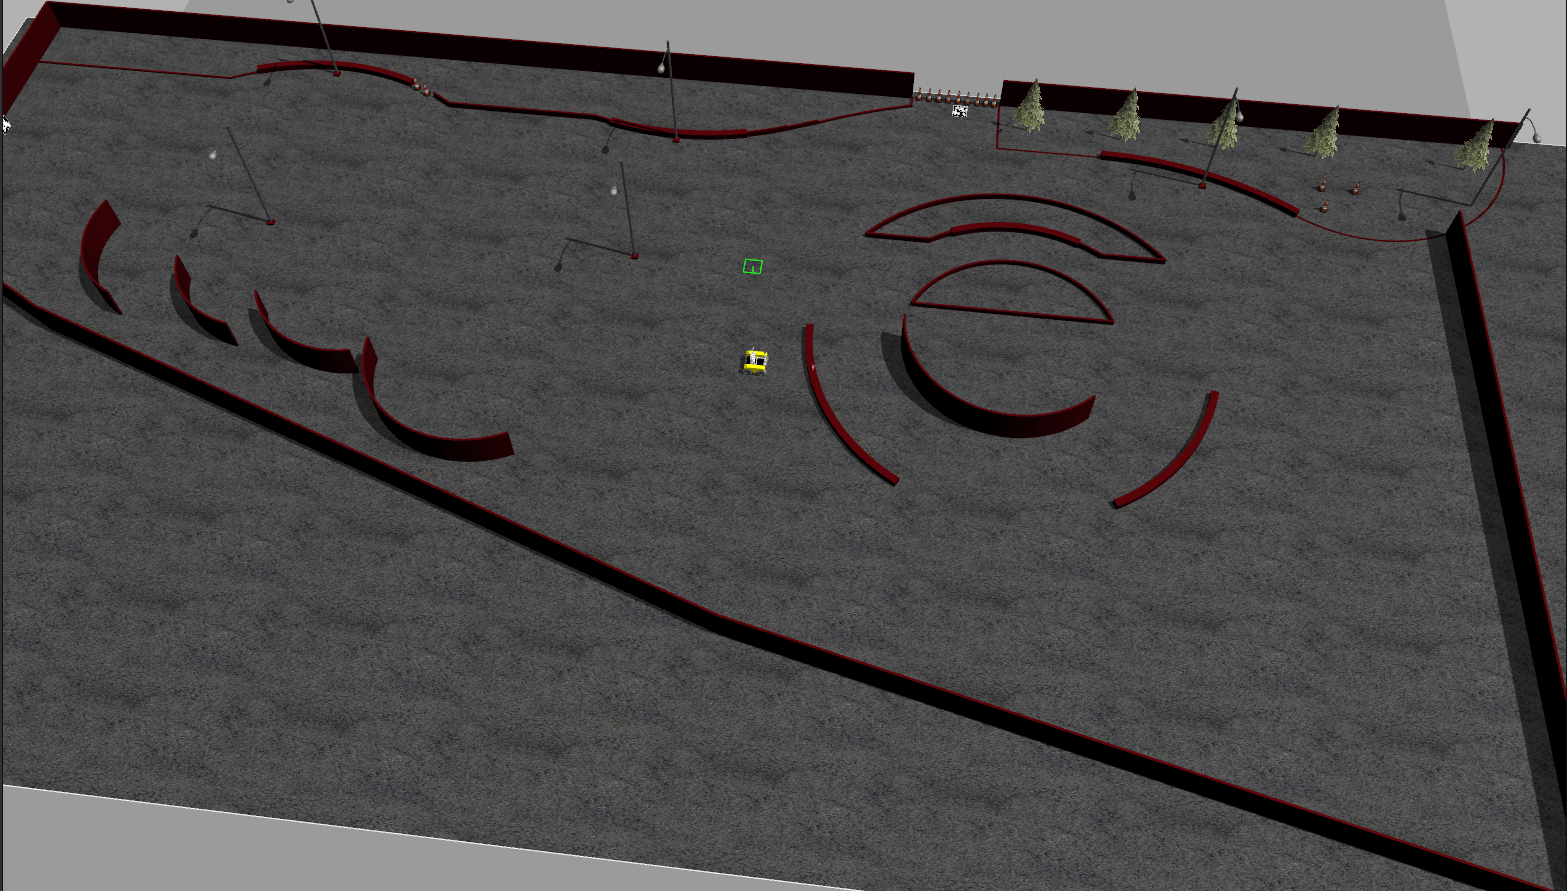
\includegraphics[width= \textwidth]{Figures/ambiente_saci.png}
%     \caption*{Fonte: Grupo de Formação em Robótica e Sistemas Autônomos}
%     \label{fig:ambiente_saci}
% \end{figure}



% \begin{figure}[H]
%     \caption{Saci modelado para simulação no \textit{Gazebo}}
%     \centering
%     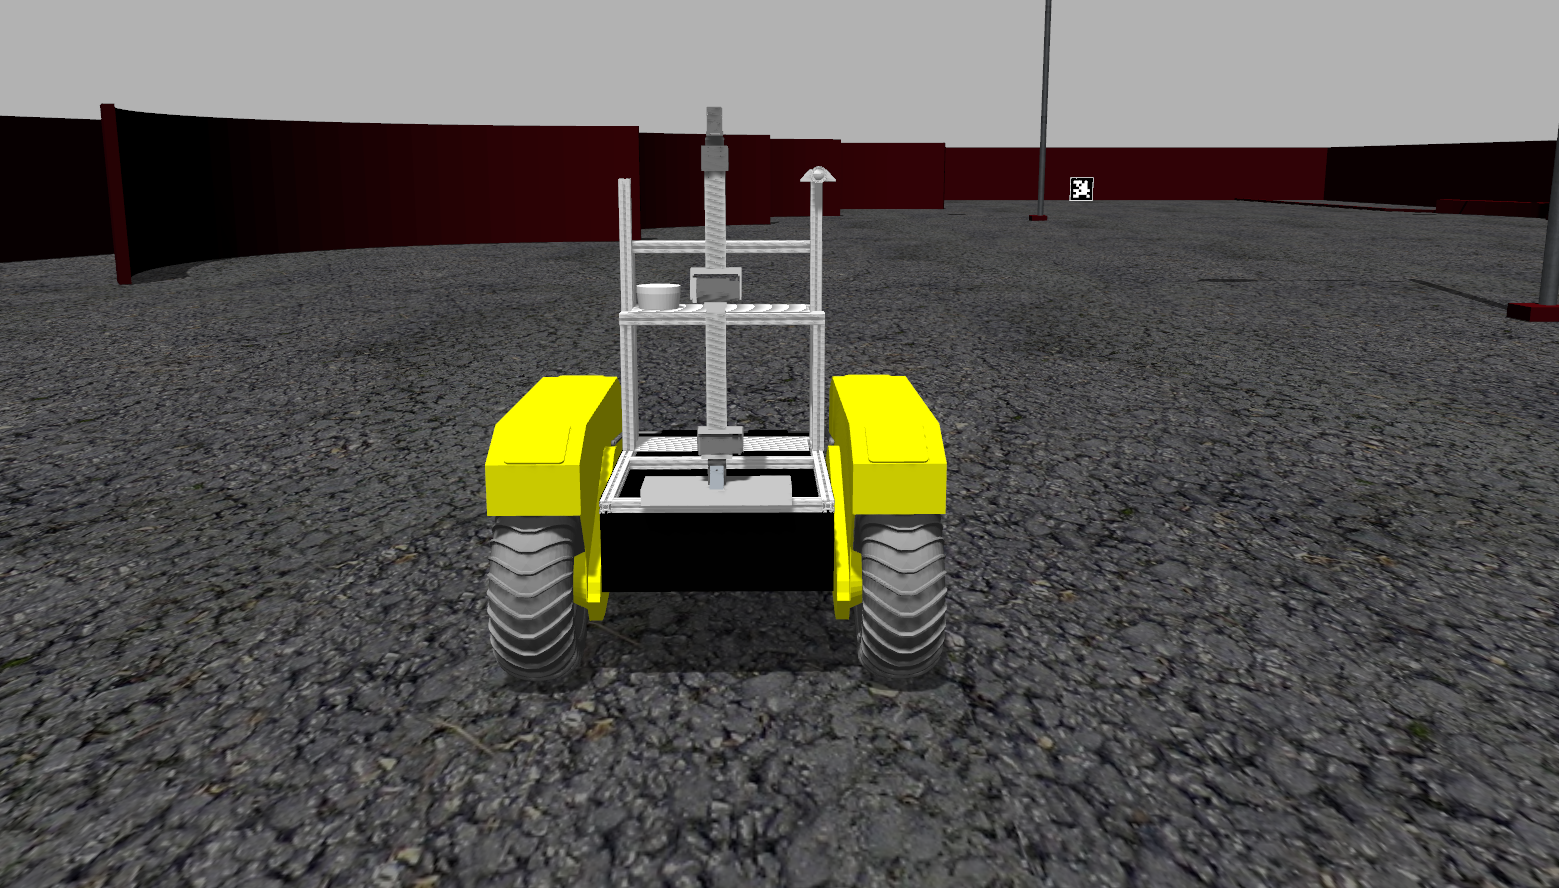
\includegraphics[width= \textwidth]{Figures/warthog_simulacao.png}
%     \caption*{Fonte: Grupo de Formação em Robótica e Sistemas Autônomos}
%     \label{fig:warthog_simulacao}
% \end{figure}


% \begin{figure}[H]
%     \caption{Modelo Real do Saci, com a identificação dos equipamentos integrados que foram utilizados}
%     \centering
%     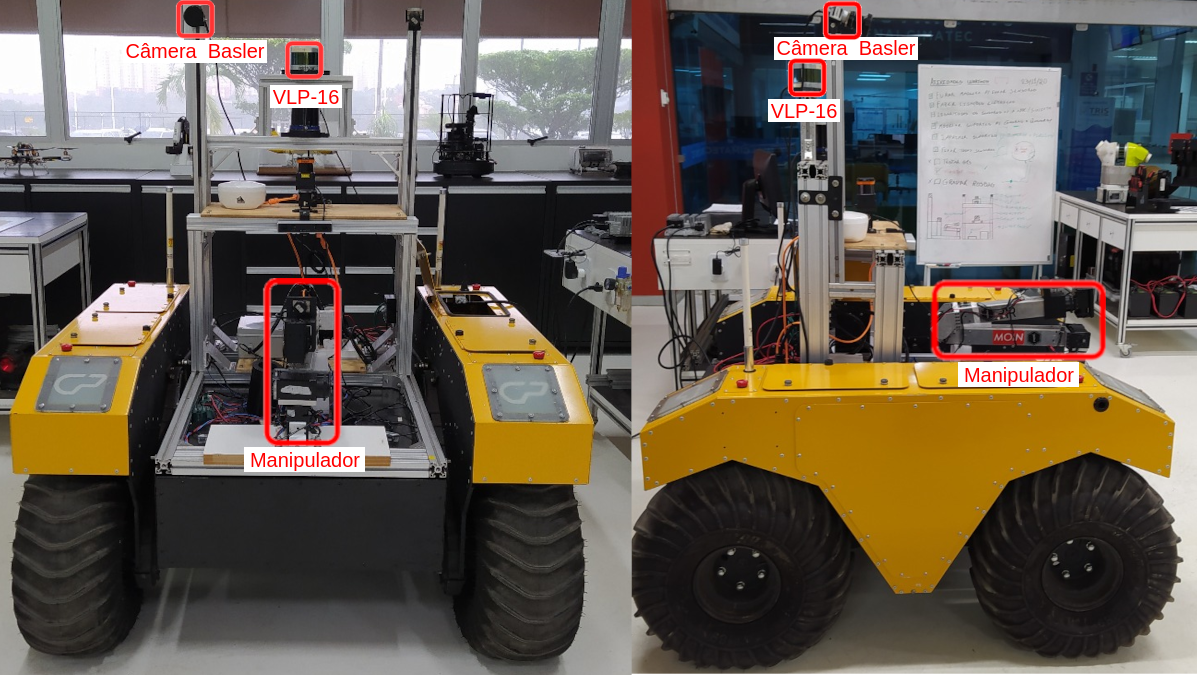
\includegraphics[width= \textwidth]{Figures/warthog_compo2.png}
%     \caption*{Fonte: Grupo de Formação em Robótica e Sistemas Autônomos}
%     \label{fig:warthog_desafio_3}
% \end{figure}


% \section{Analíse estatística R\&R da simulação do robô Darwin OP}
% \label{sec:analise_darwin}
% Teve como objetivo analisar o sistema de medição dos dados coletados durante os testes realizados nas etapas: de marcha e de revezamento do Desafio 2.5 (\ref{sec:desafio2_5}), utilizando o método de análise de variância (ANOVA). Nessa análise foi possível aplicar os conhecimentos obtidos em estatística, utilizando a ferramenta e linguagem de programação \textit{R} em um projeto realizado durante o curso, a fim de verificar o desempenho desse projeto, exemplo, a análise de precisão produzida através do estudo R\&R (Repetibilidade e Reprodutibilidade). Foram utilizadas apenas as ferramentas de simulação e para realização do estudo estatístico.
% O resultado proveniente deste estudo está descrito no documento Avaliação do Sistema de Medição- TIMON 2.5 no Apêndice \ref{append:darwinop}. Onde estão expostos dos dados coletados e a interpretação dos resultados obtidos.


